\section{Behaviour Modes}

Mode Sensitivity
\begin{itemize}
    \item Rosenberg differentiates three behavioural modes:
    \item drink: representing direct paths to the water port
    \item leave: representing direct paths to home
    \item explore: representing all other paths
    \item Modes are labeled deterministically by the following process: Start at the bout exit and step backward through the trajectory. The set of steps which monotonically increase in distance from the exit are classified as "leave". They trace a similar path from water port visits and classify these as "drink" mode. All other steps are classified as "explore".
    \item We note that this allows no room for noise. We hypothesise three types of potential noise in modes. Firstly, there may be noise due to video data parsing. Second, the mouse may make a brief error during a direct path, but continue on. Third, the mouse may be distracted during a direct path but then continue.
    \item We analyse the sensitivity of the mode classification by allowing errors of up to 5 steps, and as per Rosenberg Figure 7B, we plot the distribution of behavioural modes over time <insert figure>.
    \item We observe that differences in the distribution are negligible, concluding that despite having no error tolerance, the behavioural mode routine proposed by Rosenberg is robust.
\end{itemize}

\begin{figure}
    \centering
    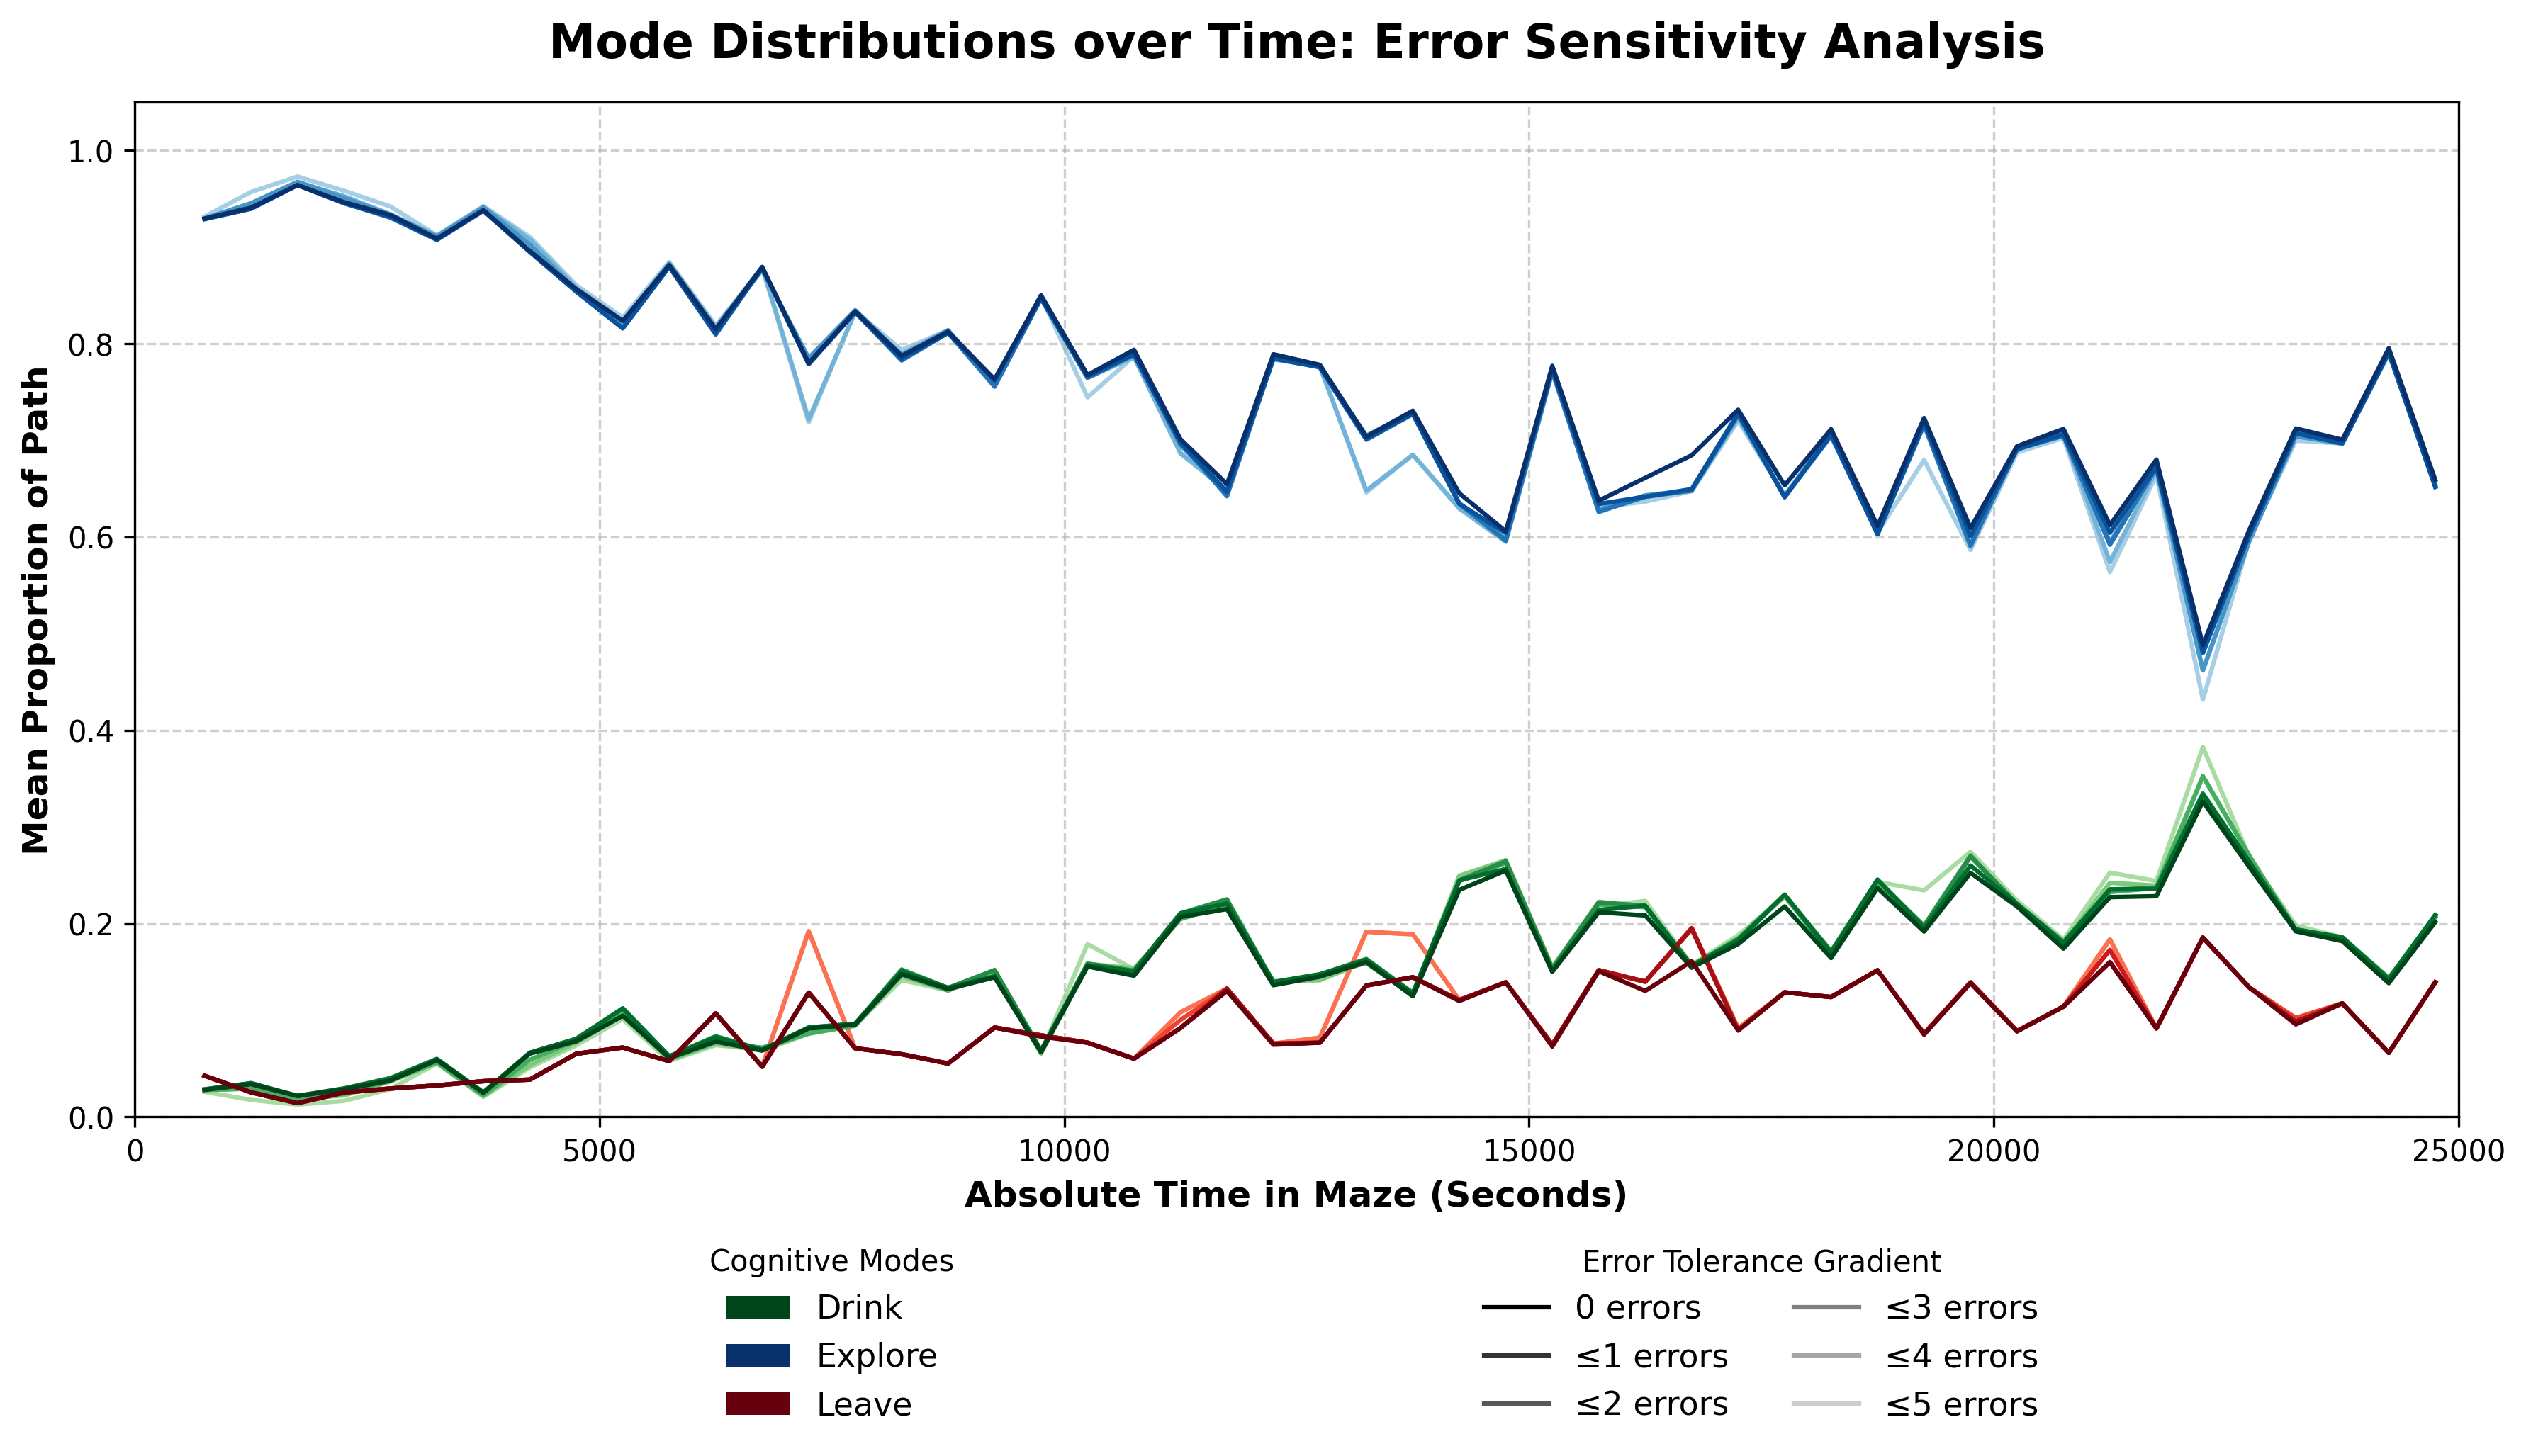
\includegraphics[width=\singlefigure]{figures/mode_sensitivity.png}
\end{figure}


